\chapter{Friedmann-Gleichung\label{chapter:thema}}
\lhead{Friedmann-Gleichung}
\begin{refsection}
\chapterauthor{Andri Hartmann und Tobias Schuler}
\printbibliography[heading=subbibliography]
\section{Expansion des Universums}
Seit langem stellte man sich die Frage, was das Universum ist und wie es sich verh"alt. Als 1912 Albert Einstein die Relativit"atstheorie herleitete, konnten gewisse Fragen beantwortet werden.
%\subsection{Kosmologische Rotverschiebung}
%Die Kosmologische Rotverschiebung ist nicht zu verwechseln mit dem Dopplereffekt. Grund daf\"{u}r ist, dass sich die Galaxien nicht in der Raumzeit voneinander entfernen, sondern sich der Raum ausdehnt. 
\subsection{Alexander Friedmann und Georges Lema\^{i}tre}
Beide entdeckten im Jahre 1927 unabh"angig voneinander die Friedmann-Lema\^{i}tre-Gleichung. Diese beschreibt das Verhalten des Universums seit dem Urknall. 
\begin{equation}
\left(\frac{a'}{a}\right) ^2 = \frac{8 \pi G}{3} \rho - \frac{k c^2}{a^2} + \frac{\Lambda c^2}{3}
\end{equation}
\subsubsection{Herleitung der Gleichung}
Um das Universum wird ein Raster gelegt. Die Einheit des Rasters wird durch den Skalenfaktor a ausgedr"uckt. Der Skalenfaktor ist abh"angig von der Zeit. Ver"andert sich das Raster, ver"andern sich auch die Positionen der Sterne und Galaxien.
\begin{figure}
	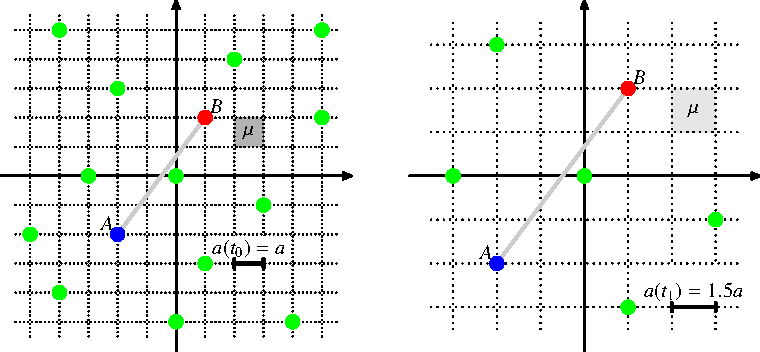
\includegraphics[width = \textwidth ]{chapters/images/friedmann-1.png}
\end{figure}
Die Distanz zwischen Punkt A und Punkt B entspricht 
\begin{equation}
D_{AB} = a(t) \sqrt{\Delta_{AB}x^2 + \Delta_{AB}y^2 + \Delta_{AB}z^2}
\end{equation}
F\"{u}r die Geschwindigkeit, mit der sich die beiden Punkte voneinander wegbewegen, gilt
\begin{equation}
v_{AB} = \dfrac{dD_{ab}}{dt} 
	   = a'(t) \sqrt{\Delta_{AB}x^2 + \Delta_{AB}y^2 + \Delta_{AB}z^2}
\end{equation}
Dabei sieht man, dass sich der Abstand in x-, y- und z-Richtung nicht ver\"{a}ndert hat und konstant bleibt. Um von diesem Abstand wegzukommen, wird die Geschwindigkeit durch die Distanz geteilt.
\begin{equation}
\frac{v_{AB} }{D_{AB}} = \frac{a'(t)}{a(t)}
\end{equation}
\begin{satz} [Hubble-Konstante]
	Die Ableitung des Skalenfaktors dividiert durch den Skalenfaktor entspricht der Hubble-Konstante.
	\begin{equation}
	\frac{a'(t)}{a(t)} = H
	\end{equation}
\end{satz}
\end{refsection}

